\documentclass[]{article}
\usepackage{lmodern}
\usepackage{amssymb,amsmath}
\usepackage{ifxetex,ifluatex}
\usepackage{fixltx2e} % provides \textsubscript
\ifnum 0\ifxetex 1\fi\ifluatex 1\fi=0 % if pdftex
  \usepackage[T1]{fontenc}
  \usepackage[utf8]{inputenc}
\else % if luatex or xelatex
  \ifxetex
    \usepackage{mathspec}
  \else
    \usepackage{fontspec}
  \fi
  \defaultfontfeatures{Ligatures=TeX,Scale=MatchLowercase}
\fi
% use upquote if available, for straight quotes in verbatim environments
\IfFileExists{upquote.sty}{\usepackage{upquote}}{}
% use microtype if available
\IfFileExists{microtype.sty}{%
\usepackage{microtype}
\UseMicrotypeSet[protrusion]{basicmath} % disable protrusion for tt fonts
}{}
\usepackage[margin=1in]{geometry}
\usepackage{hyperref}
\hypersetup{unicode=true,
            pdftitle={Emotion patterns in different lyrics genres},
            pdfborder={0 0 0},
            breaklinks=true}
\urlstyle{same}  % don't use monospace font for urls
\usepackage{color}
\usepackage{fancyvrb}
\newcommand{\VerbBar}{|}
\newcommand{\VERB}{\Verb[commandchars=\\\{\}]}
\DefineVerbatimEnvironment{Highlighting}{Verbatim}{commandchars=\\\{\}}
% Add ',fontsize=\small' for more characters per line
\usepackage{framed}
\definecolor{shadecolor}{RGB}{248,248,248}
\newenvironment{Shaded}{\begin{snugshade}}{\end{snugshade}}
\newcommand{\AlertTok}[1]{\textcolor[rgb]{0.94,0.16,0.16}{#1}}
\newcommand{\AnnotationTok}[1]{\textcolor[rgb]{0.56,0.35,0.01}{\textbf{\textit{#1}}}}
\newcommand{\AttributeTok}[1]{\textcolor[rgb]{0.77,0.63,0.00}{#1}}
\newcommand{\BaseNTok}[1]{\textcolor[rgb]{0.00,0.00,0.81}{#1}}
\newcommand{\BuiltInTok}[1]{#1}
\newcommand{\CharTok}[1]{\textcolor[rgb]{0.31,0.60,0.02}{#1}}
\newcommand{\CommentTok}[1]{\textcolor[rgb]{0.56,0.35,0.01}{\textit{#1}}}
\newcommand{\CommentVarTok}[1]{\textcolor[rgb]{0.56,0.35,0.01}{\textbf{\textit{#1}}}}
\newcommand{\ConstantTok}[1]{\textcolor[rgb]{0.00,0.00,0.00}{#1}}
\newcommand{\ControlFlowTok}[1]{\textcolor[rgb]{0.13,0.29,0.53}{\textbf{#1}}}
\newcommand{\DataTypeTok}[1]{\textcolor[rgb]{0.13,0.29,0.53}{#1}}
\newcommand{\DecValTok}[1]{\textcolor[rgb]{0.00,0.00,0.81}{#1}}
\newcommand{\DocumentationTok}[1]{\textcolor[rgb]{0.56,0.35,0.01}{\textbf{\textit{#1}}}}
\newcommand{\ErrorTok}[1]{\textcolor[rgb]{0.64,0.00,0.00}{\textbf{#1}}}
\newcommand{\ExtensionTok}[1]{#1}
\newcommand{\FloatTok}[1]{\textcolor[rgb]{0.00,0.00,0.81}{#1}}
\newcommand{\FunctionTok}[1]{\textcolor[rgb]{0.00,0.00,0.00}{#1}}
\newcommand{\ImportTok}[1]{#1}
\newcommand{\InformationTok}[1]{\textcolor[rgb]{0.56,0.35,0.01}{\textbf{\textit{#1}}}}
\newcommand{\KeywordTok}[1]{\textcolor[rgb]{0.13,0.29,0.53}{\textbf{#1}}}
\newcommand{\NormalTok}[1]{#1}
\newcommand{\OperatorTok}[1]{\textcolor[rgb]{0.81,0.36,0.00}{\textbf{#1}}}
\newcommand{\OtherTok}[1]{\textcolor[rgb]{0.56,0.35,0.01}{#1}}
\newcommand{\PreprocessorTok}[1]{\textcolor[rgb]{0.56,0.35,0.01}{\textit{#1}}}
\newcommand{\RegionMarkerTok}[1]{#1}
\newcommand{\SpecialCharTok}[1]{\textcolor[rgb]{0.00,0.00,0.00}{#1}}
\newcommand{\SpecialStringTok}[1]{\textcolor[rgb]{0.31,0.60,0.02}{#1}}
\newcommand{\StringTok}[1]{\textcolor[rgb]{0.31,0.60,0.02}{#1}}
\newcommand{\VariableTok}[1]{\textcolor[rgb]{0.00,0.00,0.00}{#1}}
\newcommand{\VerbatimStringTok}[1]{\textcolor[rgb]{0.31,0.60,0.02}{#1}}
\newcommand{\WarningTok}[1]{\textcolor[rgb]{0.56,0.35,0.01}{\textbf{\textit{#1}}}}
\usepackage{graphicx,grffile}
\makeatletter
\def\maxwidth{\ifdim\Gin@nat@width>\linewidth\linewidth\else\Gin@nat@width\fi}
\def\maxheight{\ifdim\Gin@nat@height>\textheight\textheight\else\Gin@nat@height\fi}
\makeatother
% Scale images if necessary, so that they will not overflow the page
% margins by default, and it is still possible to overwrite the defaults
% using explicit options in \includegraphics[width, height, ...]{}
\setkeys{Gin}{width=\maxwidth,height=\maxheight,keepaspectratio}
\IfFileExists{parskip.sty}{%
\usepackage{parskip}
}{% else
\setlength{\parindent}{0pt}
\setlength{\parskip}{6pt plus 2pt minus 1pt}
}
\setlength{\emergencystretch}{3em}  % prevent overfull lines
\providecommand{\tightlist}{%
  \setlength{\itemsep}{0pt}\setlength{\parskip}{0pt}}
\setcounter{secnumdepth}{0}
% Redefines (sub)paragraphs to behave more like sections
\ifx\paragraph\undefined\else
\let\oldparagraph\paragraph
\renewcommand{\paragraph}[1]{\oldparagraph{#1}\mbox{}}
\fi
\ifx\subparagraph\undefined\else
\let\oldsubparagraph\subparagraph
\renewcommand{\subparagraph}[1]{\oldsubparagraph{#1}\mbox{}}
\fi

%%% Use protect on footnotes to avoid problems with footnotes in titles
\let\rmarkdownfootnote\footnote%
\def\footnote{\protect\rmarkdownfootnote}

%%% Change title format to be more compact
\usepackage{titling}

% Create subtitle command for use in maketitle
\providecommand{\subtitle}[1]{
  \posttitle{
    \begin{center}\large#1\end{center}
    }
}

\setlength{\droptitle}{-2em}

  \title{Emotion patterns in different lyrics genres}
    \pretitle{\vspace{\droptitle}\centering\huge}
  \posttitle{\par}
    \author{}
    \preauthor{}\postauthor{}
    \date{}
    \predate{}\postdate{}
  

\begin{document}
\maketitle

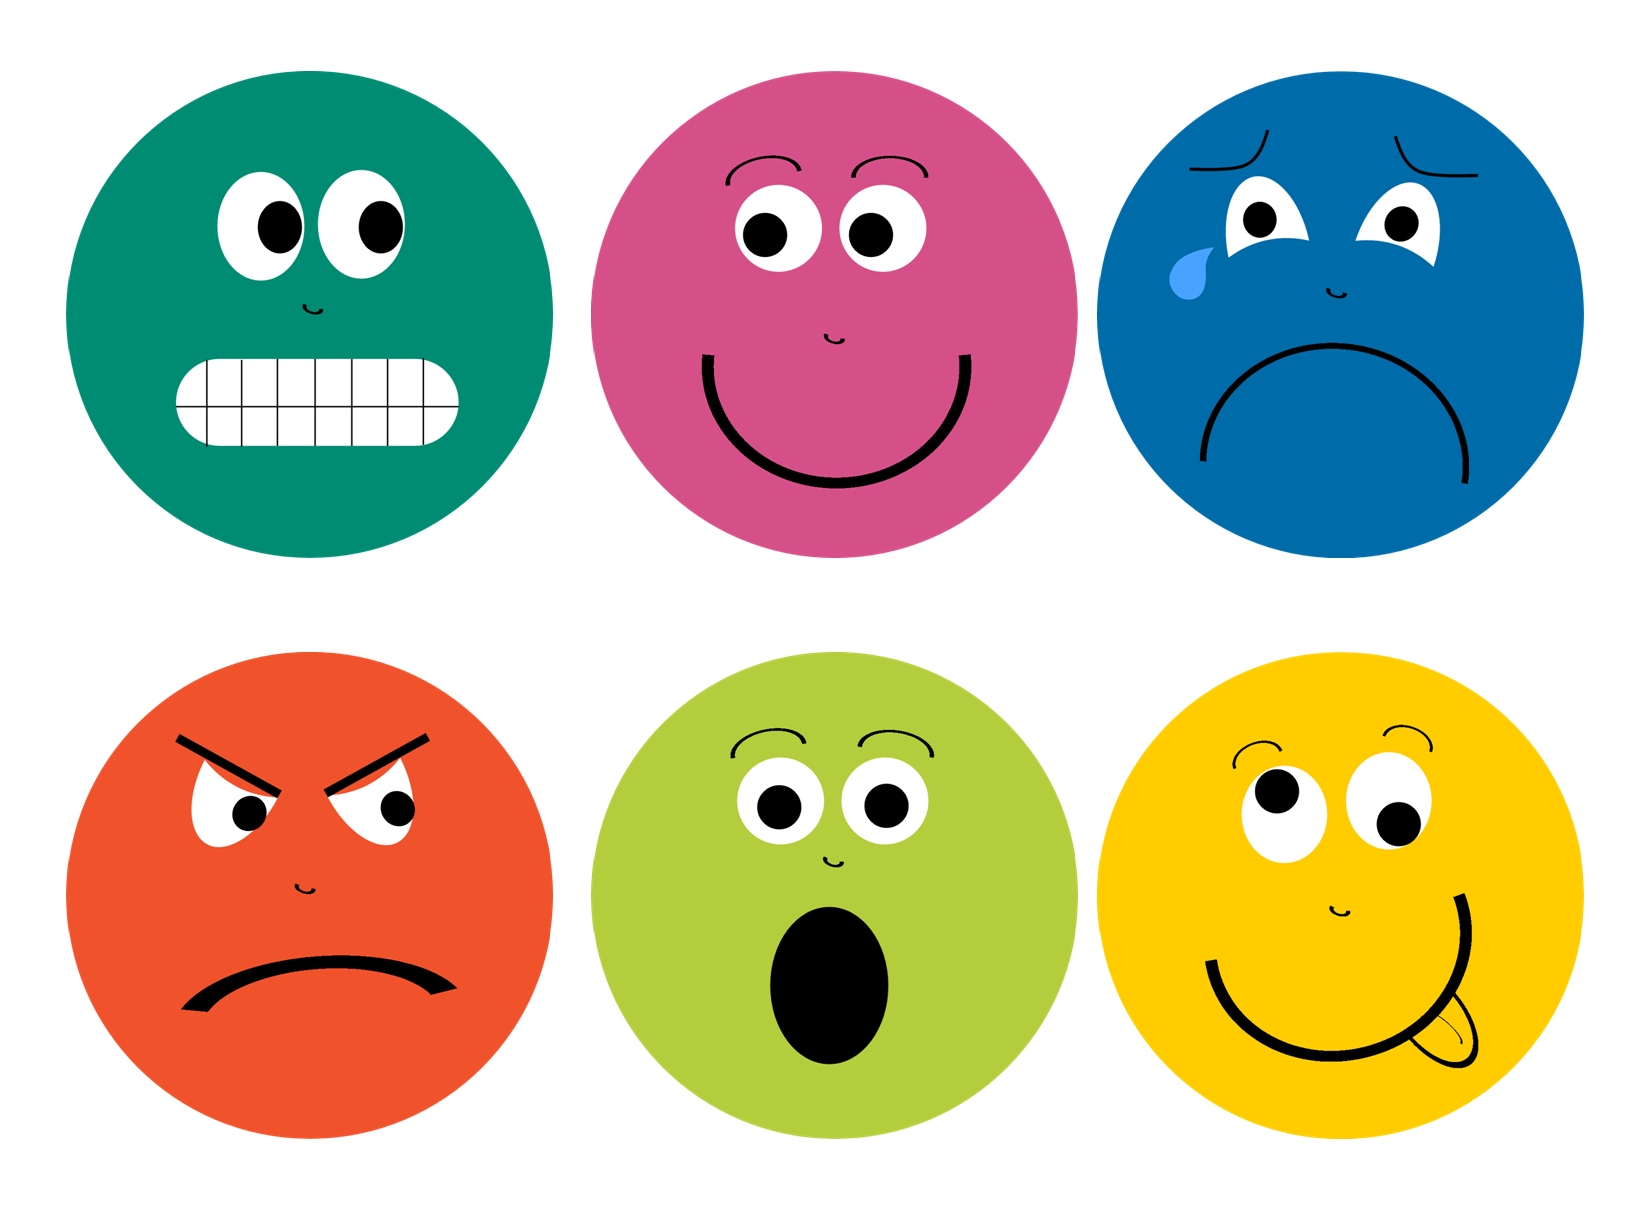
\includegraphics{D:/g/C/5243/fall2019-proj1--feichigu-master/figs/emotion.png}

\newline
\newline
\newline

We know that lyrics will contain countless emotions, anticipatoin, joy,
sadness and so on. But what will they differ in different lyrics genres,
and also in different time period? Today, my main theme is to use
sentimental analysis available in R package to explore such emotion
patterns and get some interesting findings. Basiclly, my analysis will
be conducted in three directions: 1. Compare emotions contained in words
in different lyrics genres 2. Compare emotions contained in top200 most
frequent words in different genres 3. Compare emotions contained in
words for different time period of certain genres

\begin{Shaded}
\begin{Highlighting}[]
\CommentTok{## import packages}
\KeywordTok{library}\NormalTok{(plyr)}
\KeywordTok{library}\NormalTok{(dplyr)}
\KeywordTok{library}\NormalTok{(sentimentr)}
\KeywordTok{library}\NormalTok{(syuzhet)}
\KeywordTok{library}\NormalTok{(tibble)}
\KeywordTok{library}\NormalTok{(tm)}
\KeywordTok{library}\NormalTok{(tidytext)}

\CommentTok{##load data and filter data we will not use today}
\KeywordTok{load}\NormalTok{(}\StringTok{'../output/processed_lyrics.RData'}\NormalTok{) }
\NormalTok{data =}\StringTok{ }\NormalTok{dt_lyrics}
\NormalTok{data =}\StringTok{ }\NormalTok{data }\OperatorTok\StringTok{ }\KeywordTok{filter}\NormalTok{(genre }\OperatorTok{!=}\StringTok{ 'Other'} \OperatorTok{&}\StringTok{ }\NormalTok{genre }\OperatorTok{!=}\StringTok{ 'Not Available'}\NormalTok{)}
\NormalTok{data =}\StringTok{ }\NormalTok{data }\OperatorTok\StringTok{ }\KeywordTok{filter}\NormalTok{(year}\OperatorTok{>}\DecValTok{1968}\NormalTok{)}
\CommentTok{## show counts of lyrics genres in every year}
\KeywordTok{tail}\NormalTok{(}\KeywordTok{table}\NormalTok{(data}\OperatorTok{$}\NormalTok{year,data}\OperatorTok{$}\NormalTok{genre))}
\end{Highlighting}
\end{Shaded}

\begin{verbatim}
##       
##        Country Electronic Folk Hip-Hop Indie Jazz Metal  Pop  R&B Rock
##   2011     175         85   16     382   115  103   296  791   28 1268
##   2012     163         99   28     325    89  134   261  759   40 1354
##   2013     329        156    7     276    91  195   248  712   70 1286
##   2014     252        193   28     410   104  320   309  986  100 2058
##   2015     227        137   12     212   148  168   277  588  175 1154
##   2016     194        132   19     283   115  176   260  691   50 1237
\end{verbatim}

\#\#1)Compare emotions contained in words in different lyrics genres

\begin{Shaded}
\begin{Highlighting}[]
\NormalTok{out =}\StringTok{ }\KeywordTok{matrix}\NormalTok{(}\OtherTok{NA}\NormalTok{,}\DecValTok{10}\NormalTok{,}\DecValTok{10}\NormalTok{)}
\ControlFlowTok{for}\NormalTok{ (i }\ControlFlowTok{in} \DecValTok{1}\OperatorTok{:}\DecValTok{10}\NormalTok{)\{}
\NormalTok{  fgenre =}\StringTok{ }\KeywordTok{unique}\NormalTok{(data}\OperatorTok{$}\NormalTok{genre)[i]}
\NormalTok{  fdata =}\StringTok{ }\NormalTok{data }\OperatorTok\StringTok{ }\KeywordTok{filter}\NormalTok{(genre }\OperatorTok{==}\StringTok{ }\NormalTok{fgenre)}
\NormalTok{  fsample =}\StringTok{ }\KeywordTok{sample}\NormalTok{(fdata}\OperatorTok{$}\NormalTok{stemmedwords,}\DecValTok{1000}\NormalTok{,}\DataTypeTok{replace=}\NormalTok{T)}
\NormalTok{  emotions =}\StringTok{ }\KeywordTok{get_nrc_sentiment}\NormalTok{(fsample)}
\NormalTok{  result =}\StringTok{ }\KeywordTok{colMeans}\NormalTok{(emotions)}
\NormalTok{  out[i,]  =}\StringTok{ }\NormalTok{result}
\NormalTok{\}}
\KeywordTok{colnames}\NormalTok{(out) =}\StringTok{ }\KeywordTok{colnames}\NormalTok{(emotions)}
\KeywordTok{rownames}\NormalTok{(out) =}\StringTok{ }\KeywordTok{unique}\NormalTok{(data}\OperatorTok{$}\NormalTok{genre)}
\NormalTok{out =}\StringTok{ }\KeywordTok{cbind}\NormalTok{(out,}\KeywordTok{rep}\NormalTok{(}\DecValTok{0}\NormalTok{,}\DecValTok{10}\NormalTok{))}
\KeywordTok{colnames}\NormalTok{(out)[}\DecValTok{11}\NormalTok{] =}\StringTok{ "pos_perc"}
\NormalTok{out[,}\DecValTok{11}\NormalTok{] =}\StringTok{ }\NormalTok{(out[,}\DecValTok{2}\NormalTok{]}\OperatorTok{+}\NormalTok{out[,}\DecValTok{5}\NormalTok{]}\OperatorTok{+}\NormalTok{out[,}\DecValTok{7}\NormalTok{]}\OperatorTok{+}\NormalTok{out[,}\DecValTok{8}\NormalTok{]}\OperatorTok{+}\NormalTok{out[,}\DecValTok{10}\NormalTok{])}\OperatorTok{/}\KeywordTok{rowSums}\NormalTok{(out)}\OperatorTok{*}\DecValTok{100}
\KeywordTok{print}\NormalTok{(out)}
\end{Highlighting}
\end{Shaded}

\begin{verbatim}
##            anger anticipation disgust  fear   joy sadness surprise trust
## Hip-Hop    9.470        7.011   6.445 9.256 6.513   7.712    4.845 7.914
## Pop        2.673        3.367   1.914 3.107 3.836   3.274    2.061 3.398
## Metal      5.023        3.949   3.738 6.538 3.253   5.968    2.366 3.971
## Rock       2.882        3.327   2.101 3.503 3.563   3.625    2.115 3.388
## Country    2.098        3.217   1.664 2.491 3.759   3.006    1.925 3.284
## Indie      2.278        3.047   1.797 2.968 3.278   3.368    1.902 3.200
## Jazz       1.655        2.941   1.267 2.017 3.940   2.564    1.864 2.838
## Electronic 2.474        2.892   1.730 3.119 3.063   3.083    1.713 2.824
## R&B        2.249        2.940   1.705 2.700 3.750   2.998    1.712 3.092
## Folk       3.165        3.935   2.395 3.882 4.128   4.143    2.328 3.992
##            negative positive pos_perc
## Hip-Hop      17.370   14.405 44.74110
## Pop           5.532    6.344 53.52898
## Metal        10.680    6.800 38.89951
## Rock          6.128    6.004 50.21563
## Country       4.756    5.969 56.43321
## Indie         5.404    5.499 51.69665
## Jazz          3.738    5.733 60.63662
## Electronic    5.275    5.251 50.09865
## R&B           4.731    5.804 54.60055
## Folk          6.891    7.268 51.39459
\end{verbatim}

\begin{Shaded}
\begin{Highlighting}[]
\KeywordTok{heatmap}\NormalTok{(out[,}\OperatorTok{-}\DecValTok{11}\NormalTok{],}\DataTypeTok{cexRow =}\FloatTok{0.55}\NormalTok{,}\DataTypeTok{cexCol =} \FloatTok{0.55}\NormalTok{)}
\end{Highlighting}
\end{Shaded}

\includegraphics{hw1_files/figure-latex/unnamed-chunk-2-1.pdf}

Let's forcs on the postive percentage column which represent the
percentage of positive emotions words of the genres. We can find the two
most outstanding genres are Metal and Jazz, which can represent most
negative and positive genres. Other genres, although have slight
difference in emotions' weight, stay a pos-percentage around 50\%
relatively.

\#\#2)Compare emotions contained in top200 most frequent words in
different genres

\begin{Shaded}
\begin{Highlighting}[]
\CommentTok{## First, we seperate the lyrics into words and get top200 most }
\CommentTok{## popular words in every genres}
\NormalTok{corpus <-}\StringTok{ }\KeywordTok{VCorpus}\NormalTok{(}\KeywordTok{VectorSource}\NormalTok{(dt_lyrics}\OperatorTok{$}\NormalTok{stemmedwords))}
\NormalTok{word_tibble <-}\StringTok{ }\KeywordTok{tidy}\NormalTok{(corpus) }\OperatorTok
\StringTok{  }\KeywordTok{select}\NormalTok{(text) }\OperatorTok
\StringTok{  }\KeywordTok{mutate}\NormalTok{(}\DataTypeTok{id =} \KeywordTok{row_number}\NormalTok{()) }\OperatorTok
\StringTok{  }\KeywordTok{unnest_tokens}\NormalTok{(word, text)}
\NormalTok{wordset =}\StringTok{ }\KeywordTok{matrix}\NormalTok{(}\OtherTok{NA}\NormalTok{,}\DecValTok{200}\NormalTok{,}\DecValTok{1}\NormalTok{)}
\ControlFlowTok{for}\NormalTok{ (i }\ControlFlowTok{in} \DecValTok{1}\OperatorTok{:}\DecValTok{10}\NormalTok{)\{}
\NormalTok{  fgenre =}\StringTok{ }\KeywordTok{unique}\NormalTok{(data}\OperatorTok{$}\NormalTok{genre)[i]}
\NormalTok{  c =}\StringTok{ }\KeywordTok{count}\NormalTok{(}\KeywordTok{filter}\NormalTok{(word_tibble, }
\NormalTok{                   id }\OperatorTok\StringTok{ }\KeywordTok{which}\NormalTok{(data}\OperatorTok{$}\NormalTok{genre }\OperatorTok{==}\StringTok{ }\NormalTok{fgenre)), word, }\DataTypeTok{sort =} \OtherTok{TRUE}\NormalTok{)}
\NormalTok{  wordset =}\StringTok{ }\KeywordTok{cbind}\NormalTok{(wordset,c[}\DecValTok{1}\OperatorTok{:}\DecValTok{200}\NormalTok{,}\DecValTok{1}\NormalTok{])}
\NormalTok{\}}
\NormalTok{wordset =}\StringTok{ }\NormalTok{wordset[,}\OperatorTok{-}\DecValTok{1}\NormalTok{]}
\KeywordTok{colnames}\NormalTok{(wordset) =}\StringTok{ }\KeywordTok{unique}\NormalTok{(data}\OperatorTok{$}\NormalTok{genre)}
\KeywordTok{head}\NormalTok{(wordset)}
\end{Highlighting}
\end{Shaded}

\begin{verbatim}
##   Hip-Hop   Pop Metal  Rock Country Indie  Jazz Electronic   R&B  Folk
## 1    love  love  love  love    love  love  love       love  love  love
## 2    time  time  time  time    time  time  time       time  time youre
## 3   youre youre youre youre   youre youre youre      youre youre  baby
## 4    baby  baby  baby  baby    baby   ill  baby       baby   ill  time
## 5     ill   ill   ill   ill     day   day   ill        ill  baby heart
## 6     day   day   day   day     ill heart heart        day  life   ill
\end{verbatim}

\begin{Shaded}
\begin{Highlighting}[]
\CommentTok{## Then we conduct similar sentimental analysis on the wordset to see}
\CommentTok{## what emotions do they contain}
\NormalTok{out2 =}\StringTok{  }\NormalTok{out[,}\DecValTok{1}\OperatorTok{:}\DecValTok{10}\NormalTok{]}
\ControlFlowTok{for}\NormalTok{(i }\ControlFlowTok{in} \DecValTok{1}\OperatorTok{:}\DecValTok{10}\NormalTok{)\{}
\NormalTok{  emotions =}\StringTok{ }\KeywordTok{colSums}\NormalTok{(}\KeywordTok{get_nrc_sentiment}\NormalTok{(wordset[,i]))}
\NormalTok{  out2[i,] =}\StringTok{ }\NormalTok{emotions}
\NormalTok{\}}
\NormalTok{out2 =}\StringTok{ }\KeywordTok{cbind}\NormalTok{(out2,}\KeywordTok{rep}\NormalTok{(}\DecValTok{0}\NormalTok{,}\DecValTok{10}\NormalTok{))}
\KeywordTok{colnames}\NormalTok{(out2)[}\DecValTok{11}\NormalTok{] =}\StringTok{ "pos_perc"}
\NormalTok{out2[,}\DecValTok{11}\NormalTok{] =}\StringTok{ }\NormalTok{(out2[,}\DecValTok{2}\NormalTok{]}\OperatorTok{+}\NormalTok{out2[,}\DecValTok{5}\NormalTok{]}\OperatorTok{+}\NormalTok{out2[,}\DecValTok{7}\NormalTok{]}\OperatorTok{+}\NormalTok{out2[,}\DecValTok{8}\NormalTok{]}\OperatorTok{+}\NormalTok{out2[,}\DecValTok{10}\NormalTok{])}\OperatorTok{/}\KeywordTok{rowSums}\NormalTok{(out2)}\OperatorTok{*}\DecValTok{100}
\KeywordTok{heatmap}\NormalTok{(out2[,}\OperatorTok{-}\DecValTok{11}\NormalTok{],}\DataTypeTok{cexRow =}\FloatTok{0.55}\NormalTok{,}\DataTypeTok{cexCol =} \FloatTok{0.55}\NormalTok{)}
\end{Highlighting}
\end{Shaded}

\includegraphics{hw1_files/figure-latex/unnamed-chunk-3-1.pdf}

We find Metal still get a low pos-percentage, which fits the above
analysis. And we can confirm Metal give more negative emotions than
others. The different finding is that we see folk becomes relatively
positive genre, which also make sense. However, based on the data we can
see most popular words for these genres have a lot in common, so the
emotion analysis also gave very similar outcomes. So we can't say this
analysis became so successful except it confirms Metal's sadness
pattern.

\#\#3)Compare emotions contained in words for different time period of
certain genres Because of Metal and Jazz's special patterns, I'll show
these two genres' time analysis

\begin{Shaded}
\begin{Highlighting}[]
\CommentTok{## First we seperate data into four blocks}
\NormalTok{data_metal_bef =}\StringTok{ }\NormalTok{data }\OperatorTok\StringTok{ }\KeywordTok{filter}\NormalTok{(genre}\OperatorTok{==}\StringTok{'Metal'} \OperatorTok{&}\StringTok{ }\NormalTok{year}\OperatorTok{<=}\DecValTok{2006}\NormalTok{)}
\NormalTok{data_metal_aft =}\StringTok{ }\NormalTok{data }\OperatorTok\StringTok{ }\KeywordTok{filter}\NormalTok{(genre}\OperatorTok{==}\StringTok{'Metal'} \OperatorTok{&}\StringTok{ }\NormalTok{year}\OperatorTok{>}\DecValTok{2005}\NormalTok{)}
\NormalTok{data_jazz_bef =}\StringTok{ }\NormalTok{data }\OperatorTok\StringTok{ }\KeywordTok{filter}\NormalTok{(genre}\OperatorTok{==}\StringTok{'Jazz'} \OperatorTok{&}\StringTok{ }\NormalTok{year}\OperatorTok{<=}\DecValTok{2006}\NormalTok{)}
\NormalTok{data_jazz_aft =}\StringTok{ }\NormalTok{data }\OperatorTok\StringTok{ }\KeywordTok{filter}\NormalTok{(genre}\OperatorTok{==}\StringTok{'Jazz'} \OperatorTok{&}\StringTok{ }\NormalTok{year}\OperatorTok{>}\DecValTok{2006}\NormalTok{)}
\CommentTok{## Then we get emotion scores for them and show the outcomes together}
\NormalTok{emo_metal_bef =}\StringTok{ }\KeywordTok{colMeans}\NormalTok{(}\KeywordTok{get_nrc_sentiment}\NormalTok{(data_metal_bef}\OperatorTok{$}\NormalTok{stemmedwords))}
\NormalTok{emo_metal_aft =}\StringTok{ }\KeywordTok{colMeans}\NormalTok{(}\KeywordTok{get_nrc_sentiment}\NormalTok{(data_metal_aft}\OperatorTok{$}\NormalTok{stemmedwords))}
\NormalTok{emo_metal =}\StringTok{ }\KeywordTok{rbind}\NormalTok{(emo_metal_bef,emo_metal_aft)}
\NormalTok{emo_metal =}\StringTok{ }\KeywordTok{cbind}\NormalTok{(emo_metal,}\KeywordTok{rep}\NormalTok{(}\DecValTok{0}\NormalTok{,}\DecValTok{10}\NormalTok{))}
\KeywordTok{colnames}\NormalTok{(emo_metal)[}\DecValTok{11}\NormalTok{] =}\StringTok{ "pos_perc"}
\NormalTok{emo_metal[,}\DecValTok{11}\NormalTok{] =}\StringTok{ }\NormalTok{(emo_metal[,}\DecValTok{2}\NormalTok{]}\OperatorTok{+}\NormalTok{emo_metal[,}\DecValTok{5}\NormalTok{]}\OperatorTok{+}\NormalTok{emo_metal[,}\DecValTok{7}\NormalTok{]}
                   \OperatorTok{+}\NormalTok{emo_metal[,}\DecValTok{8}\NormalTok{]}\OperatorTok{+}\NormalTok{emo_metal[,}\DecValTok{10}\NormalTok{])}\OperatorTok{/}\KeywordTok{rowSums}\NormalTok{(emo_metal)}\OperatorTok{*}\DecValTok{100}

\NormalTok{emo_jazz_bef =}\StringTok{ }\KeywordTok{colMeans}\NormalTok{(}\KeywordTok{get_nrc_sentiment}\NormalTok{(data_jazz_bef}\OperatorTok{$}\NormalTok{stemmedwords))}
\NormalTok{emo_jazz_aft =}\StringTok{ }\KeywordTok{colMeans}\NormalTok{(}\KeywordTok{get_nrc_sentiment}\NormalTok{(data_jazz_aft}\OperatorTok{$}\NormalTok{stemmedwords))}
\NormalTok{emo_jazz =}\StringTok{ }\KeywordTok{rbind}\NormalTok{(emo_jazz_bef,emo_jazz_aft)}
\NormalTok{emo_jazz =}\StringTok{ }\KeywordTok{cbind}\NormalTok{(emo_jazz,}\KeywordTok{rep}\NormalTok{(}\DecValTok{0}\NormalTok{,}\DecValTok{10}\NormalTok{))}
\KeywordTok{colnames}\NormalTok{(emo_jazz)[}\DecValTok{11}\NormalTok{] =}\StringTok{ "pos_perc"}
\NormalTok{emo_jazz[,}\DecValTok{11}\NormalTok{] =}\StringTok{ }\NormalTok{(emo_jazz[,}\DecValTok{2}\NormalTok{]}\OperatorTok{+}\NormalTok{emo_jazz[,}\DecValTok{5}\NormalTok{]}\OperatorTok{+}\NormalTok{emo_jazz[,}\DecValTok{7}\NormalTok{]}
                   \OperatorTok{+}\NormalTok{emo_jazz[,}\DecValTok{8}\NormalTok{]}\OperatorTok{+}\NormalTok{emo_jazz[,}\DecValTok{10}\NormalTok{])}\OperatorTok{/}\KeywordTok{rowSums}\NormalTok{(emo_jazz)}\OperatorTok{*}\DecValTok{100}
\KeywordTok{print}\NormalTok{(emo_metal)}
\end{Highlighting}
\end{Shaded}

\begin{verbatim}
##                  anger anticipation  disgust     fear      joy  sadness
## emo_metal_bef 5.372954     4.207405 4.005098 6.967534 3.546820 6.253019
## emo_metal_aft 5.142096     4.074552 3.788490 6.661435 3.401532 6.011211
##               surprise    trust negative positive pos_perc
## emo_metal_bef 2.566407 4.172793 11.26643 7.248189 39.09895
## emo_metal_aft 2.478886 4.044376 10.77924 6.966368 39.29977
\end{verbatim}

\begin{Shaded}
\begin{Highlighting}[]
\KeywordTok{print}\NormalTok{(emo_jazz)}
\end{Highlighting}
\end{Shaded}

\begin{verbatim}
##                 anger anticipation  disgust     fear      joy  sadness
## emo_jazz_bef 1.671419     2.918341 1.274141 2.042126 3.792612 2.491899
## emo_jazz_aft 1.635130     2.920124 1.291198 2.021714 3.854207 2.504071
##              surprise    trust negative positive pos_perc
## emo_jazz_bef 1.779650 2.802981 3.629294 5.653273 60.40425
## emo_jazz_aft 1.799147 2.853044 3.625824 5.718496 60.74849
\end{verbatim}

Together with outcomes for other genres that I didn't show here, we
conclude that there isn't an obvious change in emotions before and after
2006. But there seems to have a slight trend for positive emotions to
increase as time passed.

\#\#Summary 1. We got an emotion score table presenting emotions
contained in samples of different lyrics genres. From percentage of
positive words, we can see Metal seems to be most negative and Jazz
seems to be most positive.

\begin{enumerate}
\def\labelenumi{\arabic{enumi}.}
\setcounter{enumi}{1}
\item
  Because most popular words in these genres have many in common, we
  can't get an obvious outcome by analyzing these words' emotions.
  However, it still reinforces Metal's negative emotion and Folk become
  most positive this turn.
\item
  We use 2006 as watershed and Metal,Jazz as samples to explore emotions
  vs time. We didn't find a clear trend but they show positive emotions
  increase very slightly by the time.
\end{enumerate}


\end{document}
